\subsection{Dominion}\label{dominion}
De \emph{Dominion} module wordt gebruikt voor het aanmaken van subsites. Ga naar \drupalpath{admin/structure/dominion} voor een overzicht van alle subsites. Het aanmaken van een subsite kan serveraanpassingen vereisen. Dit is zeker het geval wanneer een SSL certificaat op een van de (sub)sites actief is.

\bigskip

\begin{center}
	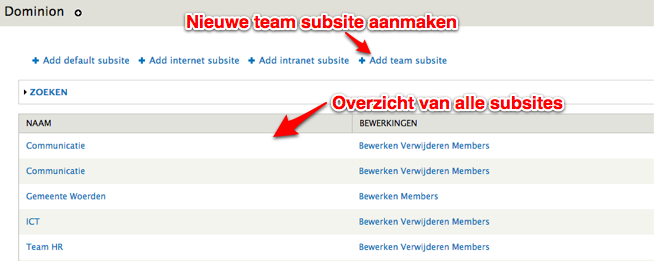
\includegraphics[width=\textwidth]{img/dominion1.png}
\end{center}

\subsubsection{Subsite toevoegen}\label{teamsubsitetoevoegen}
Wanneer een internet of intranet subsite wordt aangemaakt, dient eerst content (zoals een pagina) te worden aangemaakt die dient als de voorpagina van de subsite. Bij voorkeur is het URL van deze content coherent aan de naam van de subsite.

Klik op \emph{Add (internet/intranet/team) subsite} om een nieuwe subsite toe te voegen.

Onder \emph{Domain type} staan maximaal drie keuzes. Niet alle keuzes kunnen actief zijn.

\begin{itemize}
\item Use a subdomein of .\drupalpath{}. Hiermee kan je subsites aanmaken waarvan de naam \emph{voor} het domein gezet worden. Dat kan dus \emph{intranet}.\drupalpath{} worden.
\item Use a custom domainname. Hier kan je een eigen domein opgeven die helemaal losstaat van het huidige domein. Let wel op dat hiervoor serveraanpassingen vereist zijn.
\item Use a directory. Hiermee kan je subsites aanmaken waarvan de naam \emph{achter} het domein gezet worden. Dat kan dus \drupalpath{}\emph{intranet} worden. Wanneer deze optie geselecteerd wordt zullen er een extra opties getoond worden. Kies bij \emph{Domein} voor het domein waar het achter moet komen. Kies bij \emph{Map} de url, in het voorbeeld zou dat dus \emph{intranet} zijn. 
\end{itemize}

\bigskip

\begin{enumerate}
\item Vul bij het veld \emph{Naam} een naam in voor de subsite.
\item Kies het juiste \emph{Domain type}.
\item Specificeer eventueel de overige opties. Bij een internet of intranet subsite moet de voorpagina worden ingevuld.
\item Klik op de knop \emph{Opslaan} om de subsite toe te voegen .
\end{enumerate}

\bigskip

\begin{center}
	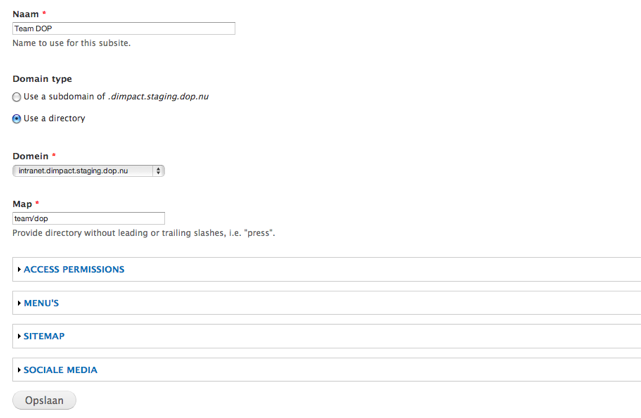
\includegraphics[width=\textwidth]{img/dominion2.png}
\end{center}

\subsubsection{Team members beheren}\label{teammembersbeheren}
Aan elke subsite kunnen \emph{Members} worden toegevoegd.

\bigskip

Klik op \emph{Members} bij de betreffende subsite om \emph{Members} toe te voegen.

\begin{center}
	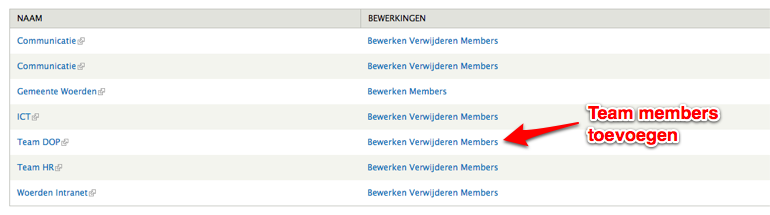
\includegraphics[width=\textwidth]{img/dominion3.png}
\end{center}

\bigskip
Op deze pagina is een lijst te vinden van de huidige teamleden.
Klik op "Add member" om een gebruiker aan de subsite toe te voegen.
Vul de gebruikersnaam of e-mail adres in, selecteer eventueel een domein specifieke rol (bijv. "teamlid") en klik vervolgens op de knop \emph{Toevoegen} om de gebruiker toe te voegen aan de lijst van \emph{Members}.

\bigskip

\begin{center}
	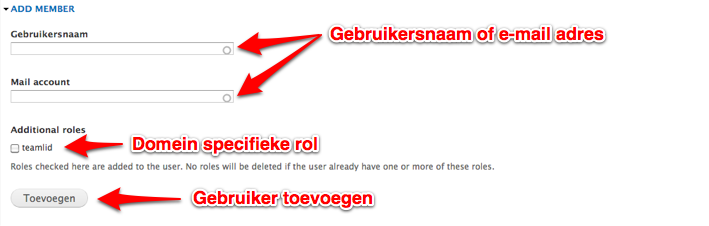
\includegraphics[width=\textwidth]{img/dominion4.png}
\end{center}
